\subsubsection{Macro-caso d'uso - Autenticazione}
\paragraph{Diagramma UML}

\begin{figure}[H]
    \centering
    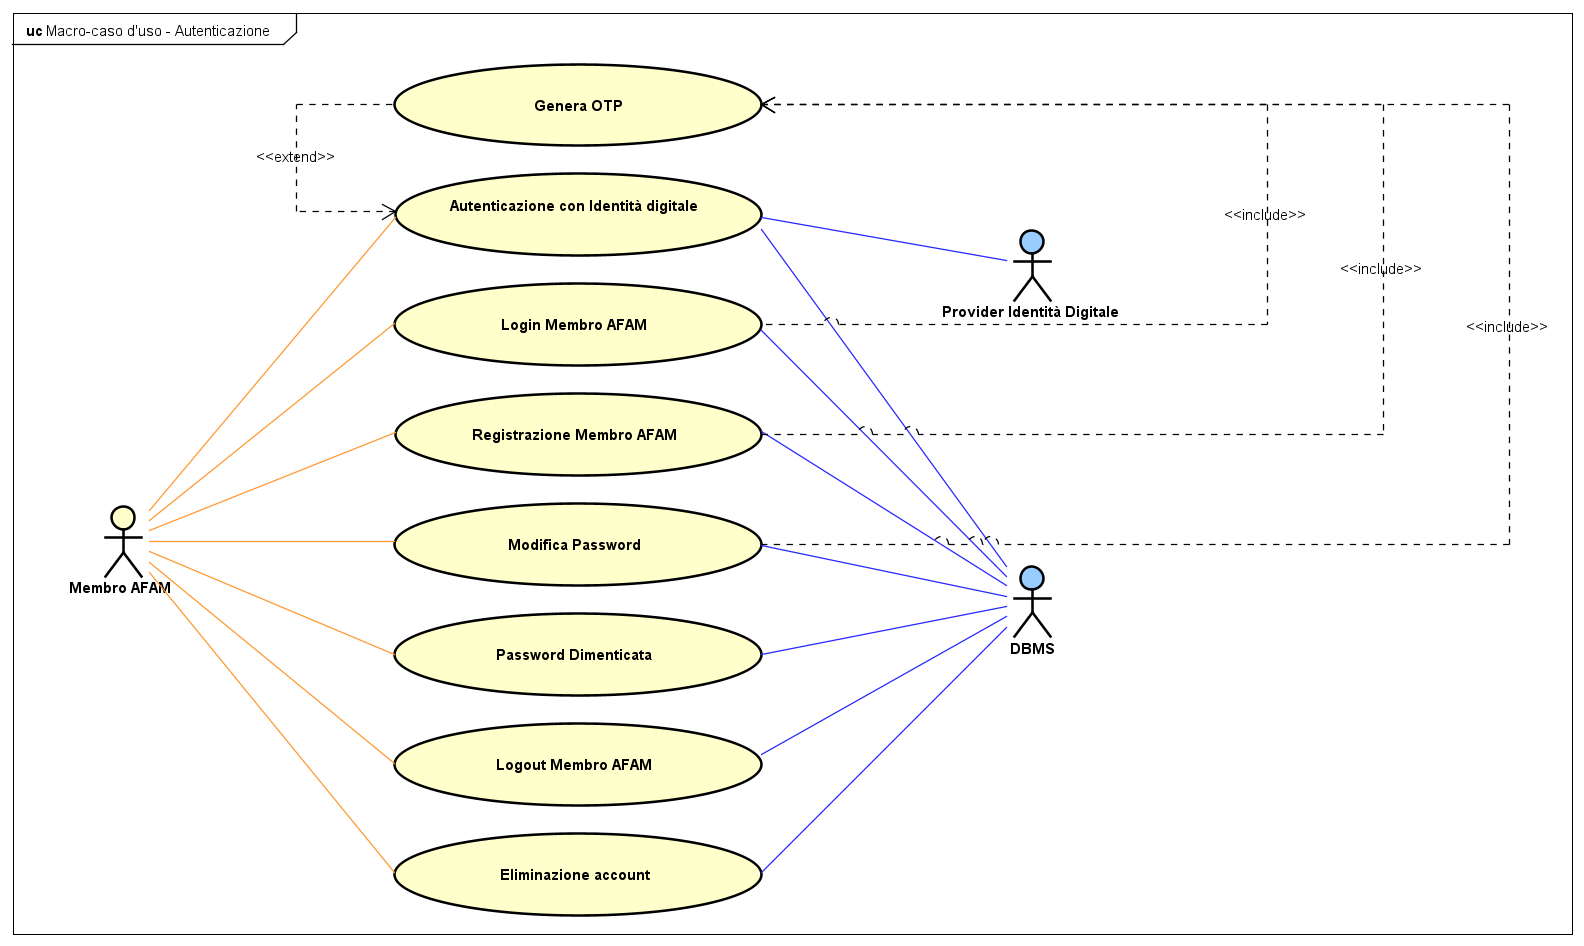
\includegraphics[width=0.95\textwidth, height=0.95\textheight, keepaspectratio]{Immagini/Use-case diagrams/Macro-caso d'uso - Autenticazione.png}
\end{figure}

\clearpage

\paragraph{Registrazione Membro AFAM}
\par{\noindent Questo caso d'uso permette a un nuovo Membro AFAM di registrarsi al sistema inserendo le proprie informazioni personali e credenziali.}

\begin{tabularx}{\textwidth}{|C|X|}
\hline
\rigaTabella{Caso d'uso}{Registrazione Membro AFAM}
\rigaTabella{ID}{REG\_MEM}
\rigaTabella{Attori}{Membro AFAM, DBMS}
\rigaTabella{Precondizione}{Il sistema ha mostrato la schermata ``WELCOME''}
\rigaTabella{Flusso degli eventi}{\begin{enumerate}
    \item Il Membro clicca sul pulsante ``REGISTRATI''
    \item Il sistema mostra a video la schermata ``REGISTRATI''
    \item Il Membro inserisce le proprie informazioni personali e le credenziali con le quali si vuole registrare all'interno del form, nonch\'e il campo di conferma della password
    \item Il Membro clicca sul pulsante ``REGISTRATI''
    \item Il sistema controlla i valori inseriti
    \item \textbf{FINCH\`E} anche solo un campo non \`e stato compilato, oppure il campo dell'email non \`e in un formato corretto, oppure anche un solo campo della password non \`e in un formato corretto, oppure se il campo della password non \`e uguale al campo di conferma, oppure l'email gi\`a esiste:
    \begin{enumerate}
        \item \textbf{SE} anche solo un campo non \`e stato compilato:
        \begin{enumerate}
            \item Il sistema mostra a video l'errore: ``Errore: Bisogna compilare tutti i campi!''
            \item Il Membro ricompila i campi
            \item Il Membro preme il pulsante ``REGISTRATI''
        \end{enumerate}
        \item \textbf{ALTRIMENTI SE} il campo dell'email non \`e in un formato corretto:
        \begin{enumerate}
            \item Il sistema mostra a video l'errore: ``Errore: Formato dell'email non corretto!'', specificando i requisiti del formato corretto
            \item Il Membro ricompila il campo
            \item Il Membro preme il pulsante ``REGISTRATI''
        \end{enumerate}
        \item \textbf{ALTRIMENTI SE} anche un solo campo della password non \`e in un formato corretto:
        \begin{enumerate}
            \item Il sistema mostra a video l'errore: ``Errore: Formato della password non corretto!'', specificando i requisiti del formato corretto
            \item Il Membro ricompila i campi
            \item Il Membro preme il pulsante ``REGISTRATI''
        \end{enumerate}
        \item \textbf{ALTRIMENTI SE} il campo della password non \`e uguale al suo campo di verifica:
        \begin{enumerate}
            \item Il sistema mostra a video l'errore: ``Errore: I campi della password devono essere uguali!''
            \item Il Membro ricompila i campi
            \item Il Membro preme il pulsante ``REGISTRATI''
        \end{enumerate}
        \item \textbf{ALTRIMENTI}:
        \begin{enumerate}
            \item Il sistema interroga il DBMS per verificare l'esistenza della mail inserita
            \item \textbf{SE} la mail inserita \`e gi\`a in uso:
            \begin{enumerate}
                \item Il sistema mostra a video l'errore: ``Errore: email gi\`a in uso! Scegline un'altra!''
                \item Il Membro ricompila i campi
                \item Il Membro preme il pulsante ``REGISTRATI''
            \end{enumerate}
        \end{enumerate}
        \item Il sistema controlla i valori inseriti
    \end{enumerate}
    \item Viene mostrato il messaggio: ``Ti arriver\`a sulla mail fornita un codice OTP da inserire. Premi OK per procedere con l'invio della mail''
    \item Viene invocato il caso d'uso ``GENERA OTP''
    \item Il sistema interroga il DBMS per inserire il nuovo Membro AFAM
    \item Il sistema autentica il nuovo Membro
    \item Il sistema mostra a video la schermata ``HOME''
\end{enumerate}
}
\rigaTabella{Postcondizione}{Il sistema ha mostrato a video la schermata ``HOME''}
\rigaTabella{Requisiti Speciali}{Le informazioni personali sono composte da: 
\begin{itemize}
    \item Nome
    \item Cognome
    \item Data di nascita
    \item Luogo di nascita
\end{itemize}
Le credenziali sono composte da: 
\begin{itemize}
    \item Email
    \item Password
    \item Conferma Password
\end{itemize}

\medskip
Il formato della password prevede almeno otto caratteri, di cui: almeno un carattere maiuscolo, almeno un carattere minuscolo, almeno un numero, almeno un carattere speciale.\newline 
Il formato dell'email prevede almeno una parola, seguita da una chiocciola, seguita da almeno un'altra parola, seguita da un punto, seguito da un dominio.}
\end{tabularx}

\clearpage

\paragraph{Login Membro AFAM}
\par{\noindent Questo caso d'uso permette a un Membro AFAM registrato di autenticarsi nel sistema tramite le proprie credenziali per accedere alla schermata Home.}

\begin{tabularx}{\textwidth}{|C|X|}
\hline
\rigaTabella{Caso d'uso}{Login Membro AFAM}
\rigaTabella{ID}{LOG\_MEM}
\rigaTabella{Attori}{Membro AFAM, DBMS}
\rigaTabella{Precondizione}{Il sistema ha mostrato la schermata ``WELCOME''}
\rigaTabella{Flusso degli eventi}{\begin{enumerate}
    \item Il Membro clicca sul pulsante ``ACCEDI''
    \item Il sistema mostra a video la schermata ``LOGIN''
    \item Il Membro inserisce le credenziali con le quali si vuole autenticare all'interno del form
    \item Il Membro clicca sul pulsante ``ACCEDI''
    \item Il sistema controlla i valori inseriti
    \item \textbf{FINCH\`E} anche solo un campo non \`e stato compilato, oppure il campo dell'email non \`e in un formato corretto, oppure il campo della password non \`e in un formato corretto, oppure le credenziali sono sbagliate:
    \begin{enumerate}
        \item \textbf{SE} anche solo un campo non \`e stato compilato:
        \begin{enumerate}
            \item Il sistema mostra a video l'errore: ``Errore: Bisogna compilare tutti i campi!''
            \item Il Membro ricompila i campi
            \item Il Membro preme il pulsante ``ACCEDI''
        \end{enumerate}
        \item \textbf{ALTRIMENTI SE} il campo dell'email non \`e in un formato corretto:
        \begin{enumerate}
            \item Il sistema mostra a video l'errore: ``Errore: Formato dell'email non corretto!'', specificando i requisiti del formato corretto
            \item Il Membro ricompila il campo
            \item Il Membro preme il pulsante ``ACCEDI''
        \end{enumerate}
        \item \textbf{ALTRIMENTI SE} il campo della password non \`e in un formato corretto:
        \begin{enumerate}
            \item Il sistema mostra a video l'errore: ``Errore: Formato della password non corretto!'', specificando i requisiti del formato corretto
            \item Il Membro ricompila il campo
            \item Il Membro preme il pulsante ``ACCEDI''
        \end{enumerate}
        \item \textbf{ALTRIMENTI}:
        \begin{enumerate}
            \item Il sistema interroga il DBMS per ottenere il Membro che possiede la coppia di credenziali inserite
            \item Il sistema effettua il controllo sull'esistenza del Membro
            \item \textbf{SE} non esiste un Membro con tali credenziali:
            \begin{enumerate}
                \item Il sistema mostra a video l'errore: ``Errore: email o password sbagliata, riprova''
                \item Il Membro ricompila i campi
                \item Il Membro clicca il pulsante ``ACCEDI''
            \end{enumerate}
        \end{enumerate}
        \item Il sistema controlla i valori inseriti
    \end{enumerate}
    \item Viene mostrato il messaggio: ``Ti arriver\`a sulla mail fornita un codice OTP da inserire. Premi OK per procedere con l'invio della mail''
    \item Viene invocato il caso d'uso ``GENERA OTP''
    \item Il sistema autentica il Membro
    \item Il sistema mostra a video la schermata ``HOME''
\end{enumerate}
}
\rigaTabella{Postcondizione}{Il sistema ha mostrato a video la schermata ``HOME''}
\rigaTabella{Requisiti Speciali}{Le credenziali sono composte da:
\begin{itemize}
    \item Email
    \item Password
\end{itemize}

\smallskip
Il formato della password prevede almeno otto caratteri, di cui: almeno un carattere maiuscolo, almeno un carattere minuscolo, almeno un numero, almeno un carattere speciale. \newline
Il formato dell'email prevede almeno una parola, seguita da una chiocciola, seguita da almeno un'altra parola, seguita da un punto, seguito da un dominio.}
\end{tabularx}

\clearpage

\paragraph{Autenticazione con Identit\`a digitale}
\par{\noindent Questo caso d'uso permette a un Membro AFAM di autenticarsi o registrarsi rapidamente nel sistema avvalendosi di un provider di identit\`a digitale (SPID).}

\begin{tabularx}{\textwidth}{|C|X|}
\hline
\rigaTabella{Caso d'uso}{Autenticazione con Identit\`a digitale}
\rigaTabella{ID}{AUT\_MEM\_ID}
\rigaTabella{Attori}{Membro AFAM, Provider Identit\`a digitale, DBMS}
\rigaTabella{Precondizione}{Il sistema ha mostrato la schermata ``LOGIN'' oppure la schermata ``REGISTRATI''}
\rigaTabella{Flusso degli eventi}{\begin{enumerate}
    \item Il Membro clicca sul pulsante ``ENTRA CON SPID''
    \item Il sistema mostra un menu con i provider di identit\`a digitale
    \item Il Membro seleziona il proprio provider
    \item Il sistema mostra a video la schermata di autenticazione del provider
    \item Il Membro si autentica
    \item \textbf{SE} l'autenticazione presso il provider non va a buon fine:
    \begin{enumerate}
        \item Il sistema mostra a video la schermata precedente
        \item Il sistema mostra a video l'errore: ``Errore: impossibile contattare il provider''
    \end{enumerate}
    \item \textbf{ALTRIMENTI}:
    \begin{enumerate}
        \item Il sistema ottiene dal provider le informazioni personali del Membro
        \item Il sistema interroga il DBMS per verificare se esiste gi\`a un membro con lo spidCode
        \item \textbf{SE} non esiste il Membro con tale spidCode:
        \begin{enumerate}
            \item Il sistema interroga il DBMS per verificare se esiste gi\`a un Membro con la mail ricevuta
            \item \textbf{SE} non esiste Membro con tale mail:
            \begin{enumerate}
                \item Il sistema interroga il DBMS per registrare il Membro con spidCode
            \end{enumerate}
            \item \textbf{ALTRIMENTI}:
            \begin{enumerate}
                \item Il sistema mostra il messaggio: ``Abbiamo trovato un account con questa email, inserire l'OTP che ti \`e stato inviato alla stessa email''
                \item Viene invocato il caso d'uso ``GENERA OTP''
                \item Il sistema interroga il DBMS per sovrascrivere i dati del Membro con quelli ricevuti dal provider e associa lo spidCode
            \end{enumerate}
        \end{enumerate}
        \item Il sistema autentica il Membro
        \item Il sistema mostra a video la schermata ``HOME''
    \end{enumerate}
\end{enumerate}
}
\rigaTabella{Postcondizione}{Il sistema ha mostrato a video la schermata ``LOGIN'' o ``REGISTRATI'' \newline \textbf{OPPURE} \newline Il sistema ha mostrato a video la schermata ``HOME''}
\rigaTabella{Requisiti Speciali}{Le informazioni personali sono composte da: 
\begin{itemize}
    \item Nome
    \item Cognome
    \item Email
    \item Codice Fiscale
    \item Data di nascita
    \item Luogo di nascita
\end{itemize}
}
\rigaTabella{Note}{Il Membro potr\`a associare all'account appena creato una password per poter accedere senza l'uso di SPID attraverso il caso d'uso ``MODIFICA PASSWORD''}
\end{tabularx}

\clearpage

\paragraph{Modifica Password}
\par{\noindent Questo caso d'uso permette a un Membro AFAM di aggiornare la propria password di accesso.}

\begin{tabularx}{\textwidth}{|C|X|}
\hline
\rigaTabella{Caso d'uso}{Modifica Password}
\rigaTabella{ID}{MOD\_PASS}
\rigaTabella{Attori}{Membro AFAM, DBMS}
\rigaTabella{Precondizione}{Il sistema ha mostrato la schermata ``GESTIONE PROFILO''}
\rigaTabella{Flusso degli eventi}{\begin{enumerate}
    \item Il Membro clicca il pulsante ``Modifica Password''
    \item Il sistema mostra la modale ``MODIFICA PASSWORD''
    \item Il Membro compila i campi ``NUOVA PASSWORD'' e ``CONFERMA NUOVA PASSWORD''
    \item Il Membro clicca il pulsante ``CONFERMA''
    \item Il sistema controlla i valori inseriti
    \item \textbf{FINCH\`E} anche un solo campo non \`e stato compilato, oppure anche un solo campo non \`e in un formato corretto, oppure il campo della password \`e diverso da quello di conferma della password:
    \begin{enumerate}
        \item \textbf{SE} anche solo un campo non \`e stato compilato:
        \begin{enumerate}
            \item Il sistema mostra a video l'errore: ``Errore: Bisogna compilare tutti i campi!''
            \item Il Membro ricompila i campi
            \item Il Membro clicca il pulsante ``CONFERMA''
        \end{enumerate}
        \item \textbf{ALTRIMENTI SE} anche un solo campo non \`e in un formato corretto:
        \begin{enumerate}
            \item Il sistema mostra a video l'errore: ``Errore: Formato della password non corretto!'', specificando i requisiti del formato corretto
            \item Il Membro ricompila i campi
            \item Il Membro clicca il pulsante ``CONFERMA''
        \end{enumerate}
        \item \textbf{ALTRIMENTI SE} il campo della nuova password non \`e uguale al suo campo di conferma:
        \begin{enumerate}
            \item Il sistema mostra a video l'errore: ``Errore: I campi ``NUOVA PASSWORD'' e ``CONFERMA NUOVA PASSWORD'' devono essere uguali!''
            \item Il Membro ricompila i campi
            \item Il Membro clicca il pulsante ``CONFERMA''
        \end{enumerate}
    \end{enumerate}
    \item Il sistema controlla i valori inseriti
    \item Il sistema mostra il messaggio: ``Ti arriver\`a sulla mail fornita un codice OTP da inserire. Premi OK per procedere con l'invio della mail''
    \item Viene invocato il caso d'uso ``GENERA OTP''
    \item Il sistema interroga il DBMS per modificare la password del Membro con la nuova password
    \item Il sistema mostra a video la schermata ``GESTIONE PROFILO''
    \item Il sistema mostra a video il messaggio: ``Password modificata correttamente''
\end{enumerate}
}
\rigaTabella{Postcondizione}{Il sistema ha mostrato a video la schermata ``HOME''}
\rigaTabella{Requisiti Speciali}{Il formato della password prevede almeno otto caratteri, di cui: almeno un carattere maiuscolo, almeno un carattere minuscolo, almeno un numero, almeno un carattere speciale.}
\hline
\end{tabularx}

\clearpage

\paragraph{Password Dimenticata}
\par{\noindent Questo caso d'uso consente a un Membro AFAM di recuperare l'accesso al proprio account richiedendo la generazione di una password temporanea inviata via email.}

\begin{tabularx}{\textwidth}{|C|X|}
\hline
\rigaTabella{Caso d'uso}{Password Dimenticata}
\rigaTabella{ID}{DIM\_PASS}
\rigaTabella{Attori}{Membro AFAM, DBMS}
\rigaTabella{Precondizione}{Il sistema ha mostrato la schermata ``LOGIN''}
\rigaTabella{Flusso degli eventi}{\begin{enumerate}
    \item Il Membro clicca sul pulsante ``Password Dimenticata?''
    \item Il sistema mostra la schermata ``RECUPERO PASSWORD''
    \item Il Membro inserisce l'email associata al suo account
    \item Il Membro preme sul pulsante ``CONFERMA''
    \item Il sistema controlla i valori inseriti
    \item \textbf{FINCH\`E} il campo dell'email \`e vuoto oppure l'email non \`e in un formato corretto:
    \begin{enumerate}
        \item \textbf{SE} il campo dell'email \`e vuoto:
        \begin{enumerate}
            \item Il sistema mostra a video l'errore: ``Errore: Bisogna compilare il campo dell'email!''
            \item Il Membro ricompila il campo
            \item Il Membro preme sul pulsante ``CONFERMA''
        \end{enumerate}
        \item \textbf{ALTRIMENTI SE} il campo dell'email non \`e in un formato corretto:
        \begin{enumerate}
            \item Il sistema mostra a video l'errore: ``Errore: L'email non \`e nel formato corretto!'', specificando i requisiti del formato corretto
            \item Il Membro ricompila il campo
            \item Il Membro preme sul pulsante ``CONFERMA''
        \end{enumerate}
    \end{enumerate}
    \item Il sistema controlla i valori inseriti
    \item Il sistema interroga il DBMS per verificare che esista un Membro con l'email inserita
    \item Il sistema effettua il controllo sulla mail
    \item \textbf{SE} esiste un Membro con la mail specificata:
    \begin{enumerate}
        \item Il sistema imposta la password del Membro ad una generata casualmente che rispetti i criteri di formato salvandola nel DBMS
        \item Il sistema manda un'email al Membro con la password appena generata
        \item Il sistema mostra a video la schermata ``LOGIN''
        \item Il sistema mostra a video il messaggio: ``Se [email] appartiene ad un account memorizzato nel sistema, ti arriver\`a una email con la tua password temporanea''
    \end{enumerate}
\end{enumerate}
}
\rigaTabella{Postcondizione}{Il sistema ha mostrato a video la schermata ``LOGIN''}
\rigaTabella{Requisiti Speciali}{Il formato dell'email prevede almeno una parola, seguita da una chiocciola, seguita da almeno un'altra parola, seguita da un punto, seguito da un dominio. \newline
L'oggetto della mail \`e: ``ARTID - NOTIFICA DI RECUPERO PASSWORD''. \newline
Il contenuto della mail \`e: ``Salve [nomeUtente], le notifichiamo che \`e stato richiesto un reset della password per il suo account di ArtID. La sua password \`e [passwordGenerata]. Le consigliamo di cambiarla una volta che effettuer\`a il prossimo accesso.''}
\hline
\end{tabularx}

\clearpage

\paragraph{Logout Membro AFAM}
\par{\noindent Questo caso d'uso permette al Membro AFAM di disconnettersi dalla piattaforma.}

\begin{tabularx}{\textwidth}{|C|X|}
\hline
\rigaTabella{Caso d'uso}{Logout Membro AFAM}
\rigaTabella{ID}{LOG\_OUT}
\rigaTabella{Attori}{Membro AFAM}
\rigaTabella{Precondizione}{Il sistema ha mostrato una qualsiasi schermata contenente l' ``HEADER''}
\rigaTabella{Flusso degli eventi}{\begin{enumerate}
    \item Il Membro clicca sul pulsante ``AZIONI PROFILO''
    \item Il sistema mostra il menu ``AZIONI PROFILO''
    \item Il Membro clicca il pulsante ``LOGOUT''
    \item Il Membro viene disconnesso
    \item Il sistema mostra a video la schermata ``LOGIN''
\end{enumerate}
}
\rigaTabella{Postcondizione}{Il sistema ha mostrato a video la schermata ``LOGIN''}
\hline
\end{tabularx}

\clearpage

\paragraph{Eliminazione Account}
\par{\noindent Questo caso d'uso permette a un Membro AFAM di eliminare il proprio profilo e tutti i materiali a esso correlati dal sistema.}


\begin{tabularx}{\textwidth}{|C|X|}
\hline
\rigaTabella{Caso d'uso}{Eliminazione Account}
\rigaTabella{ID}{DEL\_ACC}
\rigaTabella{Attori}{Membro AFAM, DBMS}
\rigaTabella{Precondizione}{Il sistema ha mostrato la schermata ``GESTIONE PROFILO''}
\rigaTabella{Flusso degli eventi}{\begin{enumerate}
    \item Il Membro preme il tasto ``CHIUDI ACCOUNT''
    \item Il sistema mostra la modale ``ELIMINA ACCOUNT''
    \item Il Membro inserisce la propria password e scrive la parola ``Elimina'' nell'apposito campo
    \item Il Membro preme il pulsante ``CONFERMA ELIMINAZIONE''
    \item Il sistema controlla i valori inseriti
    \item \textbf{FINCH\`E} almeno un campo \`e vuoto, oppure la password \`e sbagliata, oppure non c'\`e scritta la parola ``Elimina'':
    \begin{enumerate}
        \item \textbf{SE} i campi sono vuoti:
        \begin{enumerate}
            \item Il sistema mostra a video l'errore: ``Errore: Bisogna compilare tutti i campi!''
            \item Il Membro ricompila i campi
            \item Il Membro preme il pulsante ``CONFERMA ELIMINAZIONE''
        \end{enumerate}
        \item \textbf{ALTRIMENTI SE} non c'\`e scritta la parola ``Elimina'':
        \begin{enumerate}
            \item Il sistema mostra a video l'errore: ``Errore: Per confermare devi digitare esattamente la parola Elimina''
            \item Il Membro ricompila i campi
            \item Il Membro preme il pulsante ``CONFERMA ELIMINAZIONE''
        \end{enumerate}
        \item \textbf{ALTRIMENTI}:
        \begin{enumerate}
            \item Il sistema interroga il DBMS per ottenere la password del Membro
            \item Il sistema effettua il controllo sulla password
            \item \textbf{SE} la password \`e sbagliata:
            \begin{enumerate}
                \item Il sistema mostra a video l'errore: ``Errore: Password Sbagliata''
                \item Il Membro ricompila i campi
                \item Il Membro preme il pulsante ``CONFERMA ELIMINAZIONE''
            \end{enumerate}
        \end{enumerate}
        \item Il sistema controlla i valori inseriti
    \end{enumerate}
    \item Il sistema interroga il DBMS per eliminare il profilo del Membro e tutti i suoi materiali
    \item Il sistema invia una mail di conferma di avvenuta eliminazione dell'account
    \item Il sistema disconnette il Membro
    \item Il sistema mostra a video la schermata ``WELCOME''
    \item Il sistema mostra a video il messaggio: ``Account eliminato con successo''
\end{enumerate}
}
\rigaTabella{Postcondizione}{Il sistema ha mostrato a video la schermata ``WELCOME''}
\rigaTabella{Requisiti Speciali}{Se il Membro \`e autenticato con SPID e NON ha mai inserito una password, per eliminare l'account dovr\`a seguire la stessa procedura ma al posto di inserire la password si ri-autenticher\`a con spid. \newline L'oggetto della mail \`e: ``ARTID - CONFERMA ELIMINAZIONE ACCOUNT''. \newline Il contenuto della mail \`e: ``Salve [nomeUtente], la informiamo che il suo account ArtID \`e stato eliminato in data [dataEliminazione]''.}
\hline
\end{tabularx}

\clearpage

\paragraph{Genera OTP}
\par{\noindent Questo caso d'uso automatizza la generazione, il salvataggio e l'invio via email di una One-Time Password di sicurezza ogniqualvolta si compia un'azione legata ai dati sensibili.}

\begin{tabularx}{\textwidth}{|C|X|}
\hline
\rigaTabella{Caso d'uso}{Genera OTP}
\rigaTabella{ID}{GEN\_OTP}
\rigaTabella{Attori}{Membro AFAM, DBMS}
\rigaTabella{Precondizione}{Il sistema ha mostrato il messaggio di invio dell'OTP}
\rigaTabella{Flusso degli eventi}{\begin{enumerate}
    \item Il Membro clicca sul pulsante ``OK'' del messaggio mostrato a schermo
    \item Il sistema genera un OTP della durata di [durataOTP]
    \item Il sistema interroga il DBMS per salvare l'OTP
    \item Il sistema invia l'OTP alla mail del Membro
    \item Il sistema mostra a video la schermata ``VERIFICA OTP''
    \item Il Membro inserisce il codice OTP
    \item Il sistema richiede la data corrente
    \item Il sistema controlla che il codice OTP corrisponda e che non sia scaduto
    \item \textbf{FINCH\`E} il codice OTP non corrisponde o \`e scaduto:
    \begin{enumerate}
        \item Il sistema mostra a video l'errore: ``Errore: codice non valido, controlla nella mail che non sia scaduto. Se \`e scaduto clicca Riprova''
        \item Il Membro inserisce l'OTP
        \item Il sistema controlla l'OTP \label{controlla OTP}
    \end{enumerate}
    \item Il sistema mostra a video la schermata precedente
\end{enumerate}
}
\rigaTabella{Sequenze alternative}{
    \begin{enumerate}[label=9.\arabic*, start=2]
        \item Il Membro clicca sul pulsante ``RIPROVA''
        \item Il sistema genera un nuovo OTP di durata [durataOTP]
        \item Il sistema interroga il DBMS per salvare il nuovo OTP
        \item Il sistema invia l'OTP alla mail del Membro
        \item Il Membro inserisce l'OTP
    \end{enumerate}
    Il flusso riprende dal punto \ref{controlla OTP}
}
\rigaTabella{Postcondizione}{Il sistema ha mostrato a video la schermata precedente}
\rigaTabella{Requisiti Speciali}{L'oggetto della mail \`e: ``ARTID - CODICE DI ACCESSO OTP''. \newline 
Il contenuto della mail \`e: ``Salve [nomeMembro], ecco il codice d'accesso OTP. Il codice sar\`a valido fino alle [scadenzaOTP], non condividerlo con nessuno. SE NON SEI STATO TU A RICHIEDERLO NON FARE NULLA''.}
\hline
\end{tabularx}

\clearpage